\documentclass[xcolor=dvipsnames]{beamer}
\usepackage[utf8]{inputenc}
\usepackage{hyperref}
\usepackage[super]{nth} % for 1st, 2nd, etc...
\setbeamertemplate{caption}[numbered] %for figures numbering
\usepackage[export]{adjustbox} %for left and right
\usepackage{siunitx} % for degree symbol
\usepackage{graphicx}
\usepackage{subcaption}

\usetheme{CambridgeUS}


\definecolor{UBCblue}{rgb}{0.04706, 0.13725, 0.26667} % UBC Blue (primary)
\definecolor{UBCgrey}{rgb}{0, 0.46, 0.7} % UBC Grey (secondary)

\setbeamercolor{title}{bg=UBCblue,fg=white}
\setbeamercolor{frametitle}{bg=UBCblue, fg=white}
\setbeamercolor{palette primary}{bg=UBCblue,fg=white} %basso a destra
\setbeamercolor{palette secondary}{fg=UBCblue} %basso al centro
\setbeamercolor{palette tertiary}{bg=UBCgrey,fg=white} %basso e alto a sx 

\setbeamercolor{structure}{fg=UBCblue} % itemize, enumerate, etc
\setbeamercolor{section in toc}{fg=UBCblue} % TOC sections
\setbeamercolor{block title}{bg=UBCgrey!50,fg=black}
\setbeamercolor{block title example}{bg=UBCgrey!50,fg=black}

%------------------------------------------------------------
%This block of code defines the information to appear in the
%Title page
\title[Emotion Patterns in Music Playlists] %optional
{Emotion Patterns in Music Playlists}

%\subtitle{\nth{1} meeting}

\author[Sara, Mario] % (optional)
{Sara Giammusso\inst{1}\inst{2} \and Mario Guerriero \inst{1}\inst{2}}

\institute[EURECOM] % (optional)
{
 \inst{1}
 MSc student in Data Science Department, EURECOM, T\'el\'ecom ParisTech, France\\
  \inst{2}%
 MSc student in Department of Control and Computer Engineering, Politecnico di Torino, Italy
}


\date[2018 May 18] % (optional)
{Seventh Project meeting}


%End of title page configuration block
%-----------------------------------------------------------



%------------------------------------------------------------
%The next block of commands puts the table of contents at the 
%beginning of each section and highlights the current section:

\AtBeginSection[]
{
  \begin{frame}
    \frametitle{Table of Contents}
    \tableofcontents[currentsection]
  \end{frame}
}
%------------------------------------------------------------


\begin{document}

%The next statement creates the title page.
\frame{\titlepage}

%---------------------------------------------------------
%This block of code is for the table of contents after
%the title page
\begin{frame}
\frametitle{Table of Contents}
\tableofcontents
\end{frame}
%---------------------------------------------------------

\section{Introduction}
%Intoduction
\begin{frame}{Introduction}
\begin{block}{Previously On Sara\&Mario Project...}
We analyzed the SpaCy POS tagger. We added two more features: Sentiment-polarity and subjectivity and we start classifying playlists
\end{block}
Next steps:
\begin{itemize}
\item Perform the same analysis with MoodyLyrics4Q
\end{itemize}
\end{frame}

%Data Pre-processing
\section{Data Pre-processing}

%MoodyLyrics4Q Stats
\begin{frame}{MoodyLyrics4Q Stats}
\begin{figure}
  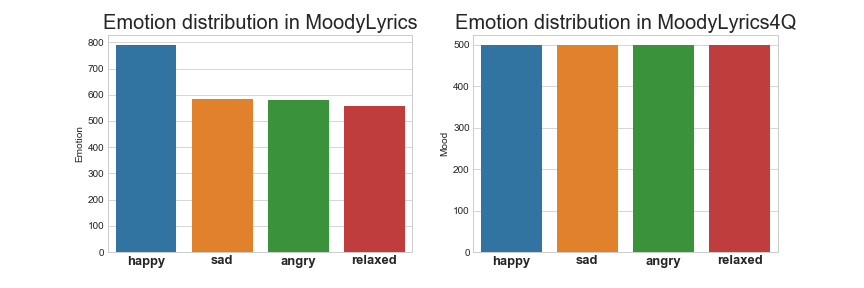
\includegraphics[width=\linewidth]{./images/Stats.png}
  \caption{Emotion Distribution in MoodyLyrics datasets}
\end{figure}
MoodyLyrics (no duplicate version): 2509 rows.\\
MoodyLyrics4Q                               : 2000 rows
Joining both datasets:                       4378 rows (46 duplicates + some songs in 4Q for which lyrics download failed)
\end{frame}

%Feature Selection
\begin{frame}{Feature Selection}
Selected Features: 
\begin{itemize}
\item Lyrics vector
\item Echoisms
\item Duplicate lines count
\item Is title in lyrics (boolean)
\item Present verb tense frequency
\item Past verb tense frequency
\item Future verb tense frequency
\item Adjectives frequency
\item Punctuation frequency
\item Sentiment polarity [-1,1]
\item Subjectivity degree [0, 1]
\end{itemize}
\end{frame}

%Classification
\section{Classification}

%Artificial Neural Network - Song Classification
\begin{frame}{Artificial Neural Network - Song Classification} 

\begin{figure}[h!]
  \centering
  \begin{subfigure}[b]{0.45\linewidth}
    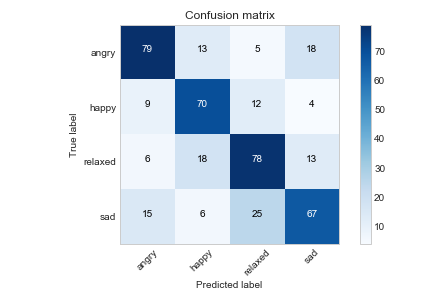
\includegraphics[width=\linewidth]{./images/CM_ANN.png}
    \caption{Test set}
  \end{subfigure}
  \begin{subfigure}[b]{0.45\linewidth}
    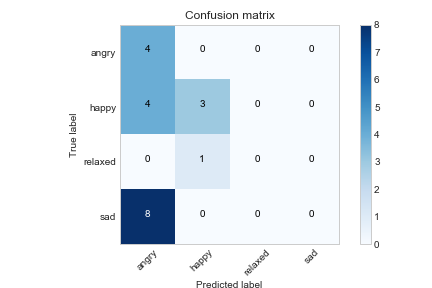
\includegraphics[width=\linewidth]{./images/CM_ANN_extra_test.png}
    \caption{Extra Test set}
  \end{subfigure}
  \caption{Confusion Matrix obtained with an ANN}
\end{figure}
Accuracy on Test: 67.12 \% \\
Accuracy on Extra Test: 35 \%
\end{frame}

%Artificial Neural Network - Playlist Classification
\begin{frame}{Artificial Neural Network - Playlist Classification}
We selected 11 playlist from 'mpd.slice.0-999.json' and we tried our model. \\
Playlist names and pids: 
\begin{itemize}
\item Relax - PID: 12
\item Relax - PID: 87
\item Relax - PID: 94
\item Feel Good - PID:656
\item Feel Good - PID: 821
\item Good Vibes - PID: 863
\item Summer 17 - PID: 612
\item Summer 2k17 - PID: 669
\item Summer country -PID: 728
\item Sad - PID: 387
\item Sad - PID: 578
\end{itemize}
Result using both datasets: 5/11\\
Result using only MoodyLyrics4Q: 8/11\\
\end{frame} 

%Logistic Regression - Song Classification
\begin{frame}{Logistic Regression  - Song Classification} 

\begin{figure}[h!]
  \centering
  \begin{subfigure}[b]{0.45\linewidth}
    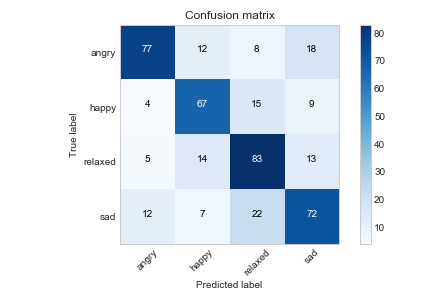
\includegraphics[width=\linewidth]{./images/CM_LR438.png}
    \caption{Test set}
  \end{subfigure}
  \begin{subfigure}[b]{0.45\linewidth}
    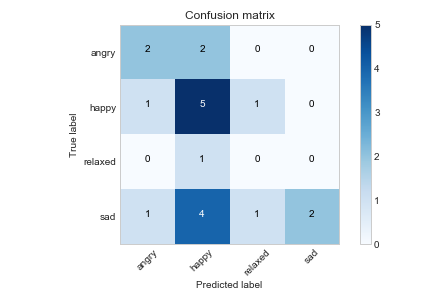
\includegraphics[width=\linewidth]{./images/CM_LR20.png}
    \caption{Extra Test set}
  \end{subfigure}
  \caption{Confusion Matrix obtained with Logistic regression}
\end{figure}
Accuracy on Test: 68 \% \\
Accuracy on Extra Test: 45 \%
\end{frame}

%SVM - Song Classification
\begin{frame}{SVM - Song Classification} 

\begin{figure}[h!]
  \centering
  \begin{subfigure}[b]{0.45\linewidth}
    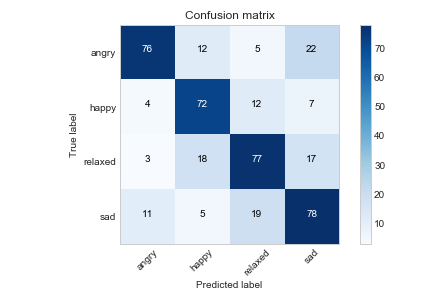
\includegraphics[width=\linewidth]{./images/CM_SVM.png}
    \caption{Test set}
  \end{subfigure}
  \begin{subfigure}[b]{0.45\linewidth}
    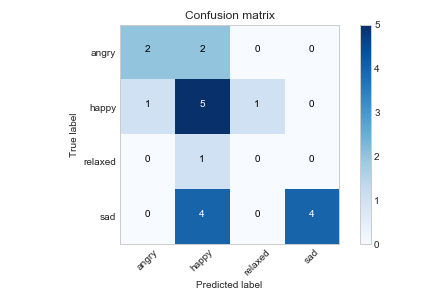
\includegraphics[width=\linewidth]{./images/CM_SVM_extra_test.png}
    \caption{Extra Test set}
  \end{subfigure}
  \caption{Confusion Matrix obtained with SVM}
\end{figure}
Accuracy on Test: 70 \% \\
Accuracy on Extra Test: 55 \%
\end{frame}



%Conclusions
\section{Conclusion}

\begin{frame}{What's next?}
Our models do not perform very good. \\
Using only MoodyLyrics4Q (instead of MoodyLyrics + MoodyLyrics4Q) is even worse. 
\begin{itemize}
\item How can we improve it? 
\end{itemize}
\end{frame}



%---------------------------------------------------------

\end{document}